% ------------------------------------------------------------
% ------------------------------------------------------------

\section{Bluetcl Reference}
\label{tcl-commands}

Bluetcl is a Tcl extension with a collection of scripts and packages 
providing an interface into the BSC view of a design.
You can execute Bluetcl commands and scripts from a
unix command line or from the command window in the Development
Workstation.

Bluetcl contains several layers (scripts, commands, packages) which
should be familiar to  the Tcl
programmer.  You can use Bluetcl extensions within Tcl scripts.
More information on Tcl is available at \te{www.tcl.tk} or
from the many books and references written about Tcl/Tk.

More information on Bluetcl can be found in the BSC documentation.

% ------------------------------------------------------------

\subsection{Invoking Bluetcl}

Bluetcl commands can be run either interactively or through Tcl
scripts.  These commands load, execute, and interact with
BSC-generated  files.   As with the Bluespec compiler,
pre-elaboration  information is obtained
from the \te{.bo} files, and post-elaboration information is
obtained from the \te{.ba} files.  

Bluetcl commands can be invoked in the following  ways.
\begin{itemize}
\item You can invoke Bluetcl from a unix prompt by typing
\te{bluetcl}.  This command provides a Tcl shell with the Bluetcl
extensions.
\item When in the BSC Development Workstation, the command window
provides a Bluetcl shell.
\item Finally, you can write and use Tcl scripts which use Bluetcl.
Examples can be found in the BSC repository.
\end{itemize}

% ------------------------------------------------------------

\subsection{Packages and namespaces}
\label{packages}
% All Bluetcl objects are defined in the namespace \te{Bluetcl}.
Bluetcl is organized into a collection of packages, which are
described in this appendix. The major packages are:
\begin{itemize}
\item The \te{Bluetcl} package which contains the low-level commands  to  interact with Bluespec files and designs.  
\item The \te{Bluesim} package containing Bluesim command extensions.\footnote{The  {\bf\tt sim} command for interacting with
Bluesim simulation objects (\te{.so} files) is contained in both the
\te{Bluetcl} and \te{Bluesim} packages.}
\item The WS package contains commands for interacting with the Workstation.
\end{itemize}

The  standard Tcl packages \te{Itcl}, \te{Itk}, and \te{Iwidgets} are
 available with Bluetcl  and can be used
 when creating  your own scripts.  

All commands in the \te{Bluetcl} package are in the \te{Bluetcl}
namespace.  All commands in the \te{Bluesim} package are in the
\te{Bluesim} namespace.   The commands in the \te{WS} package are
divided into multiple namespaces.

When referencing a command you must specify the namespace.  Example:
\begin{verbatim}
    Bluetcl::version
\end{verbatim}
Alternately, you can import commands from a namespace.  The following example
imports all the commands in a namespace:
\begin{verbatim}
    namespace import ::Bluetcl::*
\end{verbatim}
Or you can import a single command:
\begin{verbatim}
    namespace import ::Bluetcl::schedule
\end{verbatim}

Since the \te{WS} package contains multiple namespaces,  you must
specify the full namespace when referencing a \te{WS} command or
importing the commands from the namespace.  Example:
\begin{verbatim}
    WS::Build::link
    namespace import ::WS::Build::link
\end{verbatim}

Refer to the \te{Tcl} documentation for additional information on packages
and namespaces.

% ------------------------------------------------------------

\subsection{Customizing Bluetcl}
\label{custom}
\index{.bluetclrc}

You can use Bluetcl, along with all standard Tcl constructs, to
write scripts, issue commands, and customize the Development Workstation.
Bluetcl and the Development Workstation all source the setup
file \te{\$HOME/.bluetclrc} during initialization.  You can customize
Bluetcl and the Development Workstation by adding to 
 the \te{.bluetclrc} file.

% The Bluetcl interpreter is
% identical to the standard Tcl  interpreter with the
% following additions:
% \begin{itemize}
% \item It includes the Bluetcl packages
% \item The search paths are setup to look for other Bluespec
% extensions and customizations.
% \end{itemize}

The \te{namespace import} command can be put in the \te{.bluetclrc}
file, providing the command into the current namespace when the file
is sourced.  This will allow you to use just the command name in
scripts or from the command line.

% ------------------------------------------------------------

\subsection{Command Reference Conventions}

The next sections document the commands available from Bluetcl and
the Workstation (both general utilities and the Workstation code itself).
The following conventions are used within the command reference:
\begin{tabbing}
keywordandafew     \=     \kill
{\em name} \> identifier \\
{\bf keyword} \> as is \\
$[...]$ \> optional \\
%\{...\} \> repeated\\
\end{tabbing}

When an argument (or token) contains embedded spaces, the argument may
need to be enclosed in brackets (\te{\{ \}}).
% Note: For repeated arguments (\{ \}), one or more arguments may be
% specified. If only one item is specified, no brackets (\{ \}) should
% be used.  If multiple arguments are specified the list may be
% enclosed in brackets. 

% NOTE:I need a working example.  flag show seems to use a different syntax.
% Example:
% \begin{verbatim}
%      flag show sched-dot 
% This works differently - doesn't follow syntax
%      flag show sched-dot license-type p
% \end{verbatim}

% ------------------------------------------------------------

\subsection{General Bluetcl package command reference}

% -------------------------

\subsubsection{Bluetcl}

The commands in the \te{Bluetcl} package
provide a low-level interface to access BSC-specific files
(\te{.bo/.ba}) for use by Tcl programmers; they are not intended
for interactive use.  

Please refer to the BSC documentation for details on the
\te{Bluetcl} commands.

Before using a command from the \te{Bluetcl package},  the
following Tcl command must  be executed, either in a script, 
from the command line, or in the \te{.bluetclrc} file:
\begin{verbatim}
    package require Bluetcl
\end{verbatim}

All commands in the \te{Bluetcl} package are in the  \te{Bluetcl::}
namespace.  The namespace must be referenced, as described in Section
\ref{custom}, either by using the \te{namespace import} command or by
prepending the command name with \te{Bluetcl::}.  Example:
\begin{verbatim}
    Bluetcl::bpackage list
\end{verbatim}

% -------------------------

\subsubsection{Bluesim}

The \te{Bluesim} package contains the \te{sim} command which controls
Bluesim interactive mode.  This command is also found in the
\te{Bluetcl} package.

Please refer to the BSC documentation for details on the
\te{sim} command.

Before using a command from the Bluesim package,  the
following Tcl command must  be executed, either in a script, 
from the command line, or in the \te{.bluetclrc} file:
\begin{verbatim}
    package require Bluesim
\end{verbatim}

All commands in the \te{Bluesim} package are in the  \te{Bluesim::}
namespace.  The namespace must be referenced, as described in Section
\ref{custom}, either by using the \te{namespace import} command or by
prepending the command name with \te{Bluesim::}.  Example:
\begin{verbatim}
    Bluesim::sim clock
\end{verbatim}

% -------------------------

\subsubsection{Virtual}
\label{app-virtual}

The \te{Virtual} package provides Bluespec-specific accessor objects
 (virtual objects) including instantiation objects, signal objects,
 and method objects.  You  can select objects based on type, name, or
 relationship with other objects through 
 methods provided in the package.

With the \te{Virtual}  package you can:
\begin{itemize}
\item  Explore the elaborated design structure.
\item  Collect and filter the signals associated with specific
rules or submodules of a design.
\item Interact with a waveviewer object.
\item Perform these tasks in either batch or interactive mode.
\end{itemize}

Through  the design exploration capabilities of  the virtual
objects, signals associated with specific rules and instantiations can
be collected and output as a text file or  sent to a
waveform viewer.  

The term {\em virtual object} is used for two reasons:

\begin{itemize}
\item Although the objects appear to be fully populated at
  all times, the actual associated information is only obtained from
  the Bluespec database on an as-needed basis.  Caching
  mechanisms are used to avoid the need to obtain the same information
  multiple times.

\item Similarly, although objects appear  as true
  pointer-based objects, the actual implementation must conform to the
  capabilities of the \te{Tcl}  language with the \te{[incr Tcl]} (\te{iTcl})
  extensions. The \te{iTcl} package  adds   object-oriented
  programming constructs to \te{Tcl}. 
 Each object in the \te{Virtual} package is implemented as a \te{iTcl}
  class.  Information on \te{iTcl} can be 
  found at \te{www.incrtcl.sourceforge.net/itcl}

\end{itemize}

A number of the object methods select objects using   filter
patterns.  
The default pattern matching mechanism  is glob  unless the \te{-regexp} flag is
specified, specifying regular expressions. 




\subsubsubsection{inst (command)} 
\index[commands]{Virtual!inst}


The \te{inst} command provides access to the \te{inst} objects in the
current elaborated hierarchy tree.  Each object is of a defined
\te{kind}, where the values of \te{kind} are: 
\begin{itemize}
\item \te{Rule}:  Bluespec rules
\item \te{Prim}: imported Verilog IP, including common
BSC-provided primitives such as FIFOs
\item \te{Synth}:  module at the synthesis boundary
\item  \te{Inst}: not a \te{Rule}, \te{Prim}, or \te{Synth}
\end{itemize}

\begin{tabular}{|p {1.8 in}| p {3.8 in}|}
\hline
\hline
{\bf inst} {\bf top}& Returns  the top \te{inst} object or an error if
no modules have been loaded.\\
\hline
{\bf inst} {\bf filter} \te{[}{\bf -regexp}\te{]} & Returns a list of \te{inst} objects from the
current elaborated\\
   \te{[} {\bf -kind} {\em kind} \te{] [} {\bf
-nametype} {\bf bsv $\mid$ synth}\te{]} {\em pattern } & hierarchy
tree. A {\em pattern} must be specified. File
 glob matching is used for  name matching unless \te{-regexp} is
 specified, then regex is used. Optional  \te{-kind}, and \te{-nametype} flags 
 can be used to filter the results, where \te{kind} is either
 \te{Rule}, \te{Prim}, \te{Synth}, or \te{Inst} and \te{nametype}
 is either \te{bsv} or \te{synth}.  \\
\hline
\hline
\end{tabular}

{\bf Example: Using the \te{inst} command}
% Note:  The examples are generated using
% training/example/debug/DMA_ex1

The values returned from the commands are displayed in boxes.  Line
feeds have been added for clarity.


\begin{itemize}

\item   Set the
variable \te{demo} to the value returned by the \te{top} command.
\begin{verbatim}
   set demo [Virtual::inst top]
\end{verbatim}

\item Retrieve a list of the all \te{inst} objects from the
current elaborated hierarchy tree.
\begin{verbatim}
   Virtual::inst filter *
\end{verbatim}

\begin{codebox}
vInst0 vInst1 vInst2 vInst3 vInst4 vInst5 vInst6 vInst7 vInst8 vInst9
vInst10 vInst11 vInst12 vInst13 vInst14 vInst15 vInst16 vInst17
vInst18 vInst19 vInst20 vInst21 vInst22 vInst23 vInst24 vInst25
vInst26 vInst27 
\end{codebox}

\item  Display the bsv names of the \te{inst} objects. The
 \te{Virtual::omap} function is a convenience function to 
call the same method on a list of objects.  In this example, the
 method \te{name bsv} is being called for each \te{inst} returned by
 the \te{filter} method.
\begin{verbatim}
   Virtual::omap "name bsv" [Virtual::inst filter *]
\end{verbatim}

\begin{codebox}
mkDMA cnfReqF cnfRespF mmu1ReqF mmu1RespF mmu2ReqF mmu2RespF
dmaEnabledR readAddrR readCntrR currentReadR currentWriteR
portSrcDestR destAddrR responseDataF destAddrF startRead1 startRead2
finishRead1 finishRead2 startWrite1 startWrite2 finishWrite1
finishWrite2 markTransferDone writeConfig readConfig unknownConfig 
\end{codebox}

\end{itemize}


\subsubsubsection{VInst (virtual class)}

\te{VInst} is a virtual class in which  the 
\te{vinst} objects refer to  a specific instantiation in the
current elaborated hierarchy tree.

For name and path you must indicate whether you are querying the bsv
object or the synthesized object.  The name and path of an object may
be different in the BSV code and in the 
generated Verilog.  When querying for the object name and path, the
type of the object, as indicated by the
keyword \te{bsv} or \te{synth}, may be provided.  The default type is \te{bsv}.


\begin{tabular}{|p {1.8 in}| p {3.8 in}|}
\hline
\hline
{\em vinst} {\bf key}& Returns a unique identifier associated with this \te{vinst} object.\\
\hline
{\em vinst} {\bf kind}& Returns one of \te{Rule}, \te{Prim}, \te{Synth}, or \te{Inst}.\\
\hline
{\em vinst} {\bf name} \te{[}{\bf bsv $\mid$ synth}\te{]} & Returns the local
name of the instantiation, either from the bsv code or the generated
RTL.  The keyword \te{bsv} returns the name of 
the object in the BSV code while the keyword \te{synth} returns the
the  name  of the
instantiation of the object in the generated RTL.  \\
\hline
{\em vinst} {\bf path} \te{[}{\bf bsv $\mid$ synth}\te{]}& Returns the full path
name of the instantiation, either from the bsv code or the generated
RTL.  The keyword \te{bsv} returns the  path of 
the object in the BSV code while the keyword \te{synth} returns the
the  path of the
instantiation of the object in the generated RTL.  \\ 
\hline
{\em vinst} {\bf signals}& Returns a list of the
signal objects associated with the \te{vinst}.\\ % An optional \te{filter}
% argument can be used to filter the results based on a \te{signal}'s name or attributes.\\
\hline
 {\em vinst} {\bf parent}& Returns either the parent \te{vinst} object or an empty string. The top \te{vinst} does not have a parent.\\
 \hline
{\em vinst} {\bf children}& Returns a list of \te{vinst} objects.\\
\hline
{\em vinst} {\bf ancestors}&Returns a list of ancestors of the
 \te{vinst} object or an empty string.  The top \te{vinst} does not
 have any ancestors.\\
\hline
 {\em vinst} {\bf position}& Returns the position of the associated
 instantiation in the source BSV code.\\
\hline
{\em vinst} {\bf predsignals}& Returns a list of the rule predicate signals
 associated for a \te{vinst} of kind \te{Rule} or returns an empty string.\\
 \hline
{\em vinst} {\bf bodysignals}& Returns a list of the rule body signals
 associated for a \te{vinst} of kind \te{Rule} or returns an empty
 string. \\
 \hline
{\em vinst} {\bf predmethods}& Returns a list of the rule predicate methods
 associated for a \te{vinst} of kind \te{Rule} or returns an empty string.\\
 \hline
{\em vinst} {\bf bodymethods}& Returns a list of the rule body methods
 associated for a \te{vinst} of kind \te{Rule} or returns an empty
 string. \\
 \hline
{\em vinst} {\bf interface}&Returns a list of the interfaces
 associated with the \te{vinst} object.\\
\hline
% {\em vinst} {\bf module}& Returns the name of bsv module associated
% with the \te{vinst} object.\\
% \hline
 {\em vinst} {\bf portmethods}& Returns a list of all the 
 methods provided by  a \te{vinst} object
 of type \te{Prim} or \te{Synth}. \\
 \hline
{\em vinst} {\bf class}& Returns (for type checking) the {\em class} of the object (always \te{VInst}).\\
\hline
\hline
\end{tabular}

{\bf Example: Display all children}

Display the children of the top vinst, where the value of the vinst is
in the  variable \te{\$demo} (set in the previous example).

\begin{verbatim}
   $demo children
\end{verbatim}


\subsubsubsection{signal (command)}
\index[commands]{Virtual!signal}

This command provides access to the \te{signal} objects in the current
elaborated hierarchy tree and allows formatted signals to be sent to
waveform viewer or to a file for later use.

\begin{tabular}{|p {2.2 in}| p {3.4 in}|}
\hline
\hline
{\bf signal} {\bf filter}& Returns a list of \te{signal} objects from the current\\
\te{[}{\bf -inst} {\em objects} {\bf ]} \te{[}{\bf -regexp} \te{]} {\em
pattern} \te{[}{\bf -nametype} {\bf bsv $\mid$ synth}\te{]} &elaborated hierarchy tree.   The optional \te{-inst} flag specifies which
hierarchies to search.  A {\em pattern} must be specified.  File globs are used for pattern matching unless
\te{-regexp} is specified before the pattern, then regex is used.\\ 
 \hline
%   {\bf signal} {\bf add} {\em filestream} {\em signals}& Writes a list of signal objects formatted for a waveform \\
%   {\bf[ Novas\te{|}GtkWave]} {\bf[ typed\te{|}bits]}& viewer to an opened Tcl filestream.\\
\hline
\hline
\end{tabular}

{\bf Example: Using \te{signal filter}}
\begin{itemize}


\item Use the pattern \te{*} to return all signals.

\begin{verbatim}
   Virtual::signal filter *
\end{verbatim}

\begin{codebox}
vSignal0 vSignal1 vSignal2 vSignal3 vSignal4 vSignal5 vSignal6
vSignal7 vSignal8 vSignal9 vSignal10 vSignal11 vSignal12 vSignal13
vSignal14 vSignal15 vSignal16 vSignal17 vSignal18 vSignal19 vSignal20
vSignal21 vSignal22 vSignal23 vSignal24 vSignal25 vSignal26 vSignal27
vSignal28 vSignal29 vSignal30 vSignal31 vSignal32 vSignal33 vSignal34
vSignal35 vSignal36 vSignal37 vSignal38 vSignal39 vSignal40 vSignal41
vSignal42 vSignal43 vSignal44 vSignal45 vSignal46 vSignal47 vSignal48
vSignal49 vSignal50 vSignal51 vSignal52 vSignal53 vSignal54 vSignal55
vSignal56 vSignal57 vSignal58 vSignal59 vSignal60 vSignal61 vSignal62
vSignal63 vSignal64 vSignal65 vSignal66 vSignal67 vSignal68 vSignal69
vSignal70 vSignal71 vSignal72 vSignal73 vSignal74 vSignal75 vSignal76
vSignal77 vSignal78 vSignal79 vSignal80 vSignal81 vSignal82 vSignal83
vSignal84 vSignal85 vSignal86 vSignal87 vSignal88 vSignal89 vSignal90
vSignal91 vSignal92 vSignal93 vSignal94 vSignal95 vSignal96 vSignal97
vSignal98 vSignal99 vSignal100 vSignal101 vSignal102 vSignal103
vSignal104 vSignal105 vSignal106 vSignal107 vSignal108 vSignal109
vSignal110 vSignal111 vSignal112 vSignal113 vSignal114 vSignal115
vSignal116 vSignal117 vSignal118 vSignal119 vSignal120 vSignal121
vSignal122 vSignal123 vSignal124 vSignal125 vSignal126 vSignal127
vSignal128 vSignal129 vSignal130 vSignal131 vSignal132 vSignal133
vSignal134 vSignal135 vSignal136 vSignal137 vSignal138 vSignal139
vSignal140 vSignal141 vSignal142 vSignal143 vSignal144 vSignal145
vSignal146 vSignal147 vSignal148 vSignal149 vSignal150 vSignal151
vSignal152 vSignal153 vSignal154 vSignal155 vSignal156 vSignal157
vSignal158 vSignal159 vSignal160 vSignal161 vSignal162
\end{codebox}

\item Display only the \te{WILL\_FIRES} signals
\begin{verbatim}
   Virtual::signal filter WILL*
\end{verbatim}

\begin{codebox}
vSignal139 vSignal141 vSignal143 vSignal145 vSignal147 vSignal149
vSignal151 vSignal153 vSignal155 vSignal157 vSignal159 vSignal161 
\end{codebox}
\end{itemize}

% Filtering the CAN\_FIRES only under the object \te{::Vo::<inst\_19>}
% \begin{verbatim}
% % Virtual::signal filter -name CAN* -inst ::Vo::<inst_19>
% \end{verbatim}

% \begin{codebox}
% ::Vo::<signal_15>
% \end{codebox}

\subsubsubsection{VMethod (virtual class)}

The
\te{vmethod} objects  describe the methods in the current 
elaborated hierarchy. 

\begin{tabular}{|p {1.8 in}| p {3.8 in}|}
\hline
\hline
{\em  vmethod} {\bf inst}& Returns the associated \te{inst} object.\\
\hline
{\em vmethod} {\bf name}& Returns the local name of the vmethod.\\
\hline
 {\em vmethod} {\bf position}& Returns the position of the associated
 \te{inst} in the source BSV code.\\
\hline
{\em vmethod} {\bf path} {\bf bsv $\mid$ synth}& Returns the full path
name of the instantiation, either from the bsv code or the generated
RTL.  The keyword \te{bsv} returns the  path of 
the method in the BSV code while the keyword \te{synth} returns the
the  path of the
instantiation of the method in the generated RTL.  \\ 
\hline
{\em vmethod} {\bf signals}& Returns a list of the
signal objects associated with the \te{vmethod}.\\ 
\hline
{\em vmethod} {\bf class}& Returns (for type checking) the {\em class}
of the object (always \te{VMethod}).\\
\hline
\hline
\end{tabular}


\subsubsubsection{VSignal (virtual class)}

The \te{vsignal} objects describe the  signals in the current 
elaborated hierarchy. 

\begin{tabular}{|p {1.8 in}| p {3.8 in}|}
\hline
\hline
{\em  vsignal} {\bf key}& Returns a unique identifier associated with
this \te{vsignal} object.\\ 
\hline
{\em vsignal} {\bf kind}& Returns one of %\te{Input},
                                %\te{Output},\te{Clock}, 
\te{WillFire}, \te{CanFire}, or \te{Signal}.\\
\hline
{\em vsignal} {\bf name}& Returns the local name of the vsignal.\\
\hline
{\em vsignal} {\bf path} [{\bf bsv $\mid$ synth}] & Returns the full path name of the vsignal.\\
\hline
{\em vsignal} {\bf type}& Returns the BSV type of the signal.\\
\hline
{\em vsignal} {\bf inst}& Returns the associated \te{inst} object.\\
\hline
 {\em vsignal} {\bf position}& Returns the position of the associated
 \te{inst} in the source BSV code.\\
\hline
% {\em vsignal} {\bf methods}& Returns a list of all the methods associated with the \te{signal} object.\\
%\hline
{\em vsignal} {\bf class}& Returns (for type checking) the {\em class}
of the object (always \te{VSignal}).\\
% \hline
% {\em vsignal} {\bf wave\_format}& Generates the signal type and signal
% name in a format understood by the waveform viewer (\te{Waves::send\_typed\_signals}).\\ 
\hline
\hline
\end{tabular}

\subsubsubsection{reset (command)} 
\index[commands]{Virtual!reset}

\begin{tabular}{|p {1.8 in}| p {3.8 in}|}
\hline
\hline
{\bf reset}& Deletes all existing virtual objects.  This command is
called automatically when a new \te{.ba} file is loaded.\\
\hline
\hline
\end{tabular}

\subsubsubsection{omap (command)} 
\index[commands]{Virtual!omap}

\begin{tabular}{|p {1.8 in}| p {3.8 in}|}
\hline
\hline
{\bf omap}& Maps a function over a series of objects. \\
\hline
\hline
\end{tabular}


{\bf Example: Mapping the \te{name synth} command over the \te{inst filter *}}

\begin{verbatim}
   Virtual::omap "name synth" [Virtual::inst filter *]
\end{verbatim}
\begin{codebox}
cnfReqF cnfRespF mmu1ReqF mmu1RespF mmu2ReqF mmu2RespF dmaEnabledR
readAddrR readCntrR currentReadR currentWriteR portSrcDestR destAddrR
responseDataF destAddrF RL_startRead1 RL_startRead2 RL_finishRead1
RL_finishRead2 RL_startWrite1 RL_startWrite2 RL_finishWrite1
RL_finishWrite2 RL_markTransferDone RL_writeConfig RL_readConfig
RL_unknownConfig 
\end{codebox}

{\bf Example: Using  virtual objects from the Workstation}

In this example we use  virtual objects to select and display
signals on the waveform viewer.
To use the \te{Virtual} package from within the Workstation, enter the Tcl
 commands in the command window of the Workstation.   Before entering
 commannds you must bring in the \te{Virtual} package:

\begin{verbatim}
   package require Virtual
\end{verbatim}

If you optionally import all the commands from the  \te{Virtual} package you
won't have to specify the full namespace each time you reference a
command from the package:

\begin{verbatim}
   namespace import Virtual::*
\end{verbatim}


\begin{itemize}
\item Build the design and load the waveform viewer (same as with any design)

\begin{itemize}
\item Within the Workstation, load the project file, build and
simulate the design while generating a waveform dump file.

\item Open the module browser, load the top module, start and attach
the waveform viewer and load the dump file.
\end{itemize}

\item Enter the Tcl commands  in the command window of  the
Workstation.

\begin{itemize}
\item  Load and import the Virtual package
\begin{verbatim}
   package require Virtual
   namespace import Virtual::*
\end{verbatim}

\item Select all the WILL\_FIRE signals
\begin{verbatim}
   set w [signal filter WILL_FIRE*]
\end{verbatim}

\item Display the names of the WILL\_FIRE signals

\begin{verbatim}
   omap name $w
\end{verbatim}

\end{itemize}



The \te{WILL\_FIRE} signals for the  design are displayed.

\begin{codebox}
WILL_FIRE_RL_startRead1 WILL_FIRE_RL_startRead2
WILL_FIRE_RL_finishRead1 WILL_FIRE_RL_finishRead2
WILL_FIRE_RL_startWrite1 WILL_FIRE_RL_startWrite2
WILL_FIRE_RL_finishWrite1 WILL_FIRE_RL_finishWrite2
WILL_FIRE_RL_markTransferDone WILL_FIRE_RL_writeConfig
WILL_FIRE_RL_readConfig WILL_FIRE_RL_unknownConfig
\end{codebox}

\item Send the \te{WILL\_FIRE} signals to the opened wave viewer.

\begin{codebox}
   set v [WS::Wave::clone_viewer]
   $v send_objects $w
\end{codebox}

\end{itemize}



\subsubsubsection{Using Virtual objects from the command line}


                   

\begin{itemize}
\item Start bluetcl and load the top module,  \te{mkTb} in this example.  \te{rlwrap} adds
readline editing and command history.  

\begin{verbatim}
rlwrap bluetcl

   Bluetcl::flags set "-sim"
   Bluetcl::module load mkTb
\end{verbatim}

\item Load the \te{Virtual} package and set the variable \te{\$top}
equal to the top of the instance.

\begin{verbatim}
   package require Virtual
   namespace import Virtual::*
   set top [inst top]
\end{verbatim}
\begin{codebox}
vInst58
\end{codebox}

\item List the children of  the module stored in the variable
\te{\$top}.

\begin{verbatim}
   $top children
\end{verbatim}
\begin{codebox}
vInst59 vInst60 vInst61 vInst62 vInst63 vInst64 vInst65 vInst66 vInst67
\end{codebox}

\item The names listed are not very informative.  List the bsv
module name for each of the children.  

\begin{verbatim}
   foreach k [$top children] { puts [$k name bsv] }
\end{verbatim}
\begin{codebox}
initiator_0
initiator_1
target_0
target_1
dut
mkConnection
mkConnection
mkConnection
mkConnection
\end{codebox}

\item The \te{Virtual::omap} function is a convenience function to
call the same method on a list of objects.  It does approximately the
same thing as the foreach above, without  the newlines.

\begin{verbatim}
   omap "name bsv" [$top children]
\end{verbatim}
\begin{codebox}
initiator_0 initiator_1 target_0 target_1 dut mkConnection mkConnection 
mkConnection mkConnection
\end{codebox}


\item The \te{"name bsv"} class method returns the name of the objects
in the inst.   You can use a filter  to return only a certain
instances. 

\begin{verbatim}
   omap "name bsv" [inst filter *]
\end{verbatim}
\begin{codebox}
mkTb initiator_0 rand32 r reqs resps expected_resps_0 expected_resps_1
gen_reqs accept_resps_from_0 accept_resps_from_1 initiator_1 rand32 r
reqs resps expected_resps_0 expected_resps_1 gen_reqs
accept_resps_from_0 accept_resps_from_1 target_0 reqs resps respond
target_1 reqs resps respond dut from_initiator_0 from_initiator_1
to_initiator_0 to_initiator_1 to_target_0 to_target_1 from_target_0
from_target_1 initiator_0_to_target_0 initiator_1_to_target_0
initiator_0_to_target_1 initiator_1_to_target_1
target_0_to_initiator_0 target_1_to_initiator_0
target_0_to_initiator_1 target_1_to_initiator_1 mkConnection
ClientServerRequest_0 ClientServerResponse_0 mkConnection
ClientServerRequest_1 ClientServerResponse_1 mkConnection
ClientServerRequest_2 ClientServerResponse_2 mkConnection
ClientServerRequest_3 ClientServerResponse_3 
\end{codebox}

\item  Filter the above list to show only the Rules.  You can also
filter on \te{Prim, Synth, and Inst}.

\begin{verbatim}
   omap "name bsv" [inst filter * -kind Rule]
\end{verbatim}
\begin{codebox}
gen_reqs accept_resps_from_0 accept_resps_from_1 gen_reqs
accept_resps_from_0 accept_resps_from_1 respond respond
initiator_0_to_target_0 initiator_1_to_target_0
initiator_0_to_target_1 initiator_1_to_target_1
target_0_to_initiator_0 target_1_to_initiator_0
target_0_to_initiator_1 target_1_to_initiator_1 ClientServerRequest_0
ClientServerResponse_0 ClientServerRequest_1 ClientServerResponse_1
ClientServerRequest_2 ClientServerResponse_2 ClientServerRequest_3
ClientServerResponse_3 
\end{codebox}


% \item Set a variable called \te{dut}
% \begin{verbatim}
% % set dut [Virtual::inst filter * -path /main/top/dut -nametype synth]
% \end{verbatim}
% \begin{codebox}
% ::Vo::<inst_6>
% \end{codebox}

\item Find all signals and list by name (results not listed here).
\begin{verbatim}
   omap name [signal filter *]
\end{verbatim}

\item  Find all \te{WILL\_FIRE} signals and list by name (results not
listed here)

\begin{verbatim}
   omap name [signal filter WILL_FIRE*]
\end{verbatim}

\item To save the signals in a GtkWave or NovasRC file format, use the
\te{Waves} package (Section \ref{app-Waves}).
In this example we define a viewer \te{v} that is a NovasRC viewer.

\begin{verbatim}
   package require Waves
   set v [Waves::start_replay_viewer -e mkTb 
                                    -backend -sim 
                                    -viewer NovasRC 
                                    -ScriptFile x1.rc ]
\end{verbatim}

\begin{codebox}
Opening x1.rc for NovasRC script capture
novasRC1
\end{codebox}

\item Send all the \te{WILL\_FIRE} signals to the script file
\te{x1.rc}.  From the Novas viewer you will be able to load the
signals saved in the 
\te{x1.rc} file.  With the \te{Waves} package you can format, send,
and save signals to waveform and script files.
\begin{verbatim}
   $v send_objects [signal filter WILL_FIRE*]
\end{verbatim}

\end{itemize}

% -------------------------

\subsubsection{Waves}

\label{app-Waves}

The \te{Waves} package manages
waveviewer objects.  A waveviewer  is an \te{iTcl} object associated
with a specific waveform viewer instance or a waveform viewer script
file.  The \te{Waves} package contains methods and commands to  
 create   waveviewer objects and then  format,  and send
signals to those  objects.  The package also contains a scripting
functionality to  create waveviewer
script files, an executable Tcl file containing wave history
data. Waveform scripts  can be run
interactively through a waveform viewer or in batch from a command
line, for testing and verification of  designs.


To use any of the objects in the \te{Waves} package, the package
must be loaded.

\begin{verbatim}
     package require Waves
\end{verbatim}

  

You first  define a  viewer
instance which is associated with a particular waveform viewer or
waveform viewer script file.  Supported viewer types  are: \te{Novas} and \te{GtkWave}
along with their associated 
script file formats: \te{NovasRC} and \te{GtkWaveScript}.  Both the
\te{create\_viewer} and  \te{start\_replay\_viewer} commands will
define a  viewer object;  the \te{start\_replay\_viewer} 
also sets the path and opens a \te{.ba} file, assigning the viewer
object to a specific design.  

Once you have defined a viewer object, use the \te{WaveViewer} methods to
 send objects to the viewer. 
  Sent objects may be virtual
signals, instances, and methods created using the \te{Virtual}
package, described in Section \ref{app-virtual}.


\subsubsubsection{WaveViewer commands}

%\subsubsubsection{set\_nonbsv\_hierarchy (command)} 
\index[commands]{Waves!set\_nonbsv\_hierarchy}
\index[commands]{Waves!get\_nonbsv\_hierarchy}
\index[commands]{Waves!create\_viewer}

\begin{tabular}{|p {1.8 in}| p {3.8 in}|}
\hline
\hline
{\bf create\_viewer} {\em class } [{\em args}]&   Defines a virtual
viewer object of the type specified by \te{class}. The valid values for
\te{class} are \te{Novas}, \te{GtkWave}, \te{NovasRC}, and
\te{GtkWaveSript}.  The optional \te{args}  are
shown in Figure \ref{Wavestcl} and the table below.\\
\hline
{\bf start\_replay\_viewer} [{\em args}] & Defines a virtual viewer
object ready to use on a specific design (sets the path and opens the
\te{.ba} file.)  The optional \te{args}  are
shown in Figure \ref{Wavestcl} and the tables below.   Refer to the
\te{WaveViewer} section for more options.\\
\hline
{\bf set\_nonbsv\_hierarchy} {\em hierarchy}&Sets the Verilog
hierarchy as default for all new viewers.  The default is \te{/main/top}. \\
\hline
{\bf get\_nonbsv\_hierarchy}&Returns the value of the Verilog hierarchy. \\
\hline
\hline
\end{tabular}

The abstract class in the package is the \te{WaveViewer} class hierarchy.  The classes \te{Viewer}
and \te{ScriptFile} define specific types of viewers and inherit  the
methods and attributes defined in the  \te{WaveViewer} class, 
  shown in Figure \ref{Wavestcl}.  Additional arguments,
specific to either viewers or script files, are defined in those
respective classes.


\subsubsubsection{Configure arguments}

The \te{iTcl} \te{configure} method provides access to public variables as
 configuration options and a method for setting  values of the
 variables.  These variables can also be modified when a replay
 script is run or the \te{start\_replay\_viewer} method is called.
The following  arguments are used by the
\te{configure} method to configure the waveviewer.  The table is divided
into sections by classes.  The \te{WaveViewer} arguments are used by
all classes, while the \te{Viewer} and \te{ScriptFile} arguments are used
by their respective classes. 


\begin{figure}[htb]
\begin{center}
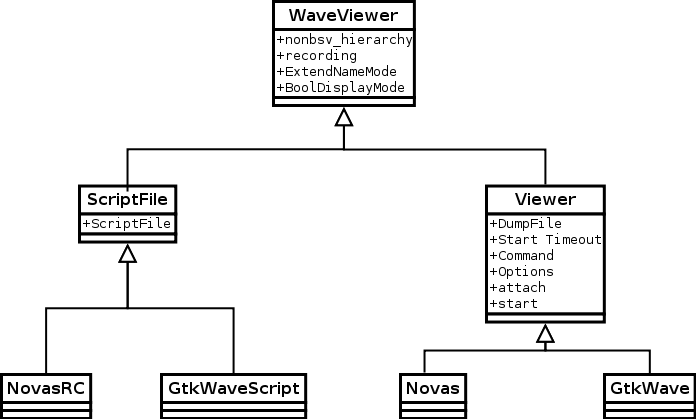
\includegraphics[width = 5 in]{figures/Wavestcl}
\caption{Inheritance of WaveViewer Class}
\label{Wavestcl}
\end{center}
\end{figure}





\begin{tabular}{|p {2.0 in}| p {3 in}|p{.6in}|}
\hline

\multicolumn{3}{|c|}{Configure arguments}\\
\hline

Argument&Description&Default  \\
\hline\hline
\multicolumn{3}{|l|}{ Arguments for all WaveViewer classes}\\
\hline
\hline
 \te{-nonbsv\_hierarchy} {\em path}&  Verilog hierarchy &\te{/main/top}\\

%\hline
 \te{-ExtendNameMode} {\bf true$\mid$false}&Determines how names are displayed in the viewer&
 false \\
%\hline
\te{-BoolDisplayMode} {\bf true$\mid$false} &Display Boolean as enum (true/false) or as 1/0 &false \\
%\hline 
\te{-recording} {\bf true$\mid$false}&If true,  commands are always recording &true\\
\hline
 \multicolumn{3}{|l|}{Arguments for Viewer classes (Novas and GtkWave)}\\
 \hline
\te{-DumpFile} {\em file}&Name of the dump file&\\
%\hline
\te{-StartTimeout} {\em time}&Delay after starting before declaring a timeout
 (Specific to viewer).  The {\em time} is an Integer.&20\\
%\hline
\te{-Command} {\em command}&Command to start viewer&\\
%\hline
\te{-Options} {\em options} &Command line options provided to viewer&\\

\te{-start} [{\bf 0} $\mid$ {\bf 1}]& Starts the wave viewer &0\\
\te{-attach} {\em viewer} &Attaches to the viewer& \\
\hline
 \multicolumn{3}{|l|}{Arguments for ScriptFile classes (NovasRc and GtkWaveScript)}\\
 \hline
\te{-ScriptFile} {\em file} & Specifies the name of the script file.&\\
\hline
\hline
\end{tabular}


\subsubsubsection{WaveViewer methods} 

\te{WaveViewer} is a virtual class in which the \te{viewer} objects
 refer to a specific instantiation of a
 waveform viewer or script file object.   
The  methods allow you to  configure, control, and query the \te{viewer}
 object.   You can send virtual objects and signals directly to the
 the viewer or   save the wave history  as a \te{.tcl} script file.



\begin{tabular}{|p {1.8 in}| p {3.8 in}|}
\hline
\hline
{\em viewer} {\bf configure} {\em args} & Uses the \te{iTcl}
\te{configure} method to set the configuration options.\\
\hline
{\em viewer} {\bf start} {\em args}& Starts the wave viewer object with the
provided {\em args}.  The arguments are listed in the \te{Configure
Arguments} table.\\
\hline
{\em viewer} {\bf isRunning}&Returns \te{true} if the wave viewer object is running.\\
\hline
{\em viewer} {\bf attach} {\em waveviewer} &Attaches the selected wave viewer
object.  If empty, detaches.\\
\hline
{\em viewer} {\bf close}&Closes the selected wave viewer object.\\
\hline
{\em viewer} {\bf load\_dump\_file} {\em filename} & Loads the file
{\em filename}
into the wave viewer object.\\
\hline
{\em viewer} {\bf reload\_dump\_file} &Reloads the current dump file.\\
\hline
{\em viewer} {\bf dump\_file\_loaded}&Returns \te{true} if the dump file is loaded. \\
\hline
{\em viewer} {\bf send\_objects} {\em objects}& Sends  virtual objects of type
\te{VInst}, \te{VSignal}, or \te{VMethod}  to the wave viewer object.\\
\hline
{\em viewer} {\bf send\_instance} {\em vinst} [{\em modifier}] & Sends an instance
object with a modifier to the wave viewer object.  The valid values of
\te{modifier} are \te{CLK, QOUT, CANFIRE, WILLFIRE, ALL, PREDICATE,
BODY}.  The default is \te{ALL}. \\
\hline
{\em viewer} {\bf send\_signals} {\em signal} & Sends the signal name (string of
the Verilog name) to the wave viewer.\\
\hline
{\em viewer} {\bf save\_history} {\em filename} &Saves the wave send history to a
tcl script file (\te{.tcl}) \\
\hline
{\em viewer} {\bf replay\_history\_file} {\em filename} & Replays the script file on
the wave viewer, sourcing the waveviewer script file without creating
a \te{wave\_history} file.\\
\hline
 {\em viewer} {\bf replay\_history\_list} {\em history\_list} &Replays the history
list. When a waveviewer script file is sourced it creates  a list variable named
\te{wave\_history}. Use  this method to replay the \te{wave\_history} file.\\
\hline
\hline
\end{tabular}




\subsubsubsection{WaveViewer script file}
\index{script file}


 The waveviewer script file is an
executable Tcl (\te{.tcl}) file containing wave history data. 
  The script file contains a list of
\te{wave\_history} elements where  each  element is comprised of  a
tag, a name, and a 
code value.  The tags are described in the table below.  The name is
the signal name and  can
contain  wildcards allowing signals to be selected dynamically when the file is
sourced or executed.  The data in the code value is based on the type
of signal.   The file  can be edited or
manipulated by the user in a text editor. 

The script file is created through the \te{save\_history} method.  You
can replay the script file using \te{replay\_history\_file}, which
will source the \te{.tcl} file and display the wave history on the
specified viewer instance.   You can also source the \te{.tcl} file 
from a bluetcl shell, creating a list variable named
\te{wave\_history} and then    replay the saved \te{\$wave\_history}
file through the \te{replay\_history\_list} method.


\begin{tabular}{|p{1 in}|p{4.5in}|}
\hline
\multicolumn{2}{|c|}{WaveViewer Script File Tags}\\
\hline
Tag& Signal Description\\
\hline \hline
\te{VSignal}& \te{VSignal}  object generated by the \te{Virtual}
class. \\
\hline
\te{SSignal} &Simple signal name.\\
\hline
\te{TSignal}&Simple signal name where the type is stored in the code value.\\
\hline
\te{VInst}&\te{VInst} object generated by the \te{Virtual} class.\\
\hline
\end{tabular}


The following options, in addition to the configure options,  are used when running the replay script or the
\te{start\_replay\_viewer} method.


\begin{tabular}{|p {1.8 in}|p{3.8in}|}
\hline
\multicolumn{2}{|c|}{Options for running  replay script and
\te{start\_replay\_viewer} method}\\ 
% \hline
% Option&Description  \\
\hline\hline
\te{-help} & Lists the options for the method  \\
\te{-p} {\em path}& Sets the Bluespec search path\\
\te{-e} {\em module}& Specifies the top  module\\
\te{-backend} [{\bf -verilog $\mid$ -sim}]& Specifies Verilog or Bluesim
as the backend, defaults to -verilog if left blank.\\

\te{-viewer} {\em class}&Sets the viewer class.   The valid values
for \te{class} are \te{Novas}, \te{GtkWave}, \te{NovasRC}, and
\te{GtkWaveSript}.\\
\hline
\hline

\end{tabular}



The script file can be either executed in a Unix shell or sourced in a
Tcl shell.   Executing the
script file from a Unix shell will execute the
following steps:
\begin{enumerate}
\item Load the \te{.ba} files (this may take some time)
\item Start the viewer
\item Execute the history
\item Exit
\end{enumerate}

\subsubsubsection{Example:  Creating and executing a viewer script file}

\begin{itemize}

\item Start bluetcl.  The command line in the Workstation is also a
bluetcl shell.

\begin{verbatim}
rlwrap bluetcl
\end{verbatim}

\item Load the \te{Virtual} and \te{Waves} packages.

\begin{verbatim}
   package require Virtual
   package require Waves
\end{verbatim}

\item Define the viewer and name it \te{v}

\begin{verbatim}
   set v [Waves::start_replay_viewer -e mkTb 
                                    -backend -sim 
                                    -viewer NovasRC 
                                    -ScriptFile x1.rc ]
\end{verbatim}

\begin{codebox}
Opening x1.rc for NovasRC script capture
novasRC1
\end{codebox}

\item Set the variable \te{r} to all rules where the name ends in 1

\begin{verbatim}
   set r [Virtual::inst filter -kind Rule *1]
\end{verbatim} 

\begin{codebox}
vInst17 vInst26 vInst44 vInst45 vInst48 vInst49 vInst52 vInst53
\end{codebox}

\item These are the instance names.  Let's view the BSV names
\begin{verbatim}
   Virtual::omap "name bsv" $r
\end{verbatim}

\begin{codebox}
accept_resps_from_1 accept_resps_from_1 initiator_0_to_target_1
initiator_1_to_target_1 target_0_to_initiator_1
target_1_to_initiator_1 ClientServerRequest_1 ClientServerResponse_1 
\end{codebox}

\item Send the objects in \te{\$r} to  to the viewer file \te{\$v} (\te{x1.rc})
\begin{verbatim}
   $v send_objects $r
\end{verbatim}

\item Save the session as a \te{WaveViewer} (\te{.tcl)} script file
\begin{verbatim}
   $v save_history x1.tcl
\end{verbatim}
\end{itemize}

\subsubsubsection{Example: Replaying a script on a waveform viewer}

\begin{itemize}
\item Start bluetcl and load the \te{Virtual} and \te{Waves} packages

\item Define a Novas viewer 

\begin{verbatim}
   set v1 [Waves::start_replay_viewer -e mkTb -backend -sim -viewer Novas]
\end{verbatim}

\item Start the viewer and load the dump file
\begin{verbatim}
   $v1 start
   $v1 load_dump_file dump.vcd
\end{verbatim}

\item Souce the \te{x1.tcl} file created in the previous example.
This will create the file \te{wave\_history}.
\begin{verbatim}
   source x1.tcl
\end{verbatim}

\item Replay the wave history

\begin{verbatim}
   $v1 replay_history_list $wave_history
\end{verbatim}

\item The waves will be displayed on the waveform viewer.

\end{itemize}

\subsubsubsection{Example: Loading a saved waveform file from within
the Workstation}

With a saved waveform files you can easily save and load a set of
signals through multiple iterations of a design, easily comparing
changes from one iteration to the next.

To load the saved signal files (\te{x1.rc})  using the Workstation:
\begin{itemize}
\item Open the design in the Workstation

\item Open the Module Browser

\item {\bf Load} top module

\item {\bf Start} the waveform viewer

\item {\bf Load} the dump file

\item From the waveviewer, restore signal ({\bf File $\rightarrow$ 
Restore Signal} in Novas).  Select the saved signals (\te{x1.rc}).

\item The waves will be displayed on the waveform viewer.
\end{itemize}

The above steps could all be done from a bluetcl command line, within
or outside of the Workstation.

% \subsubsection{Executing a \te{WaveViewer} script file}

% In the example above, we saved our session as a script file named
% \te{x1.tcl}.  

% \begin{enumerate}

% \end{enumerate}

% ------------------------------------------------------------

\subsection{Workstation package command reference}
 The \te{WS} package provides a
programming interface  to customize
the Workstation.  Specifically,  commands available from the Workstation menus
and toolbars can be executed from the Workstation command line or  included in \te{Tcl} scripts which are executed
from the Workstation.   These commands are only available in the
Workstation.  Attempting to use them in Bluetcl will
result in an error.

Tcl scripts using \te{WS} commands must be added to the
\index{.bluetclrc} \te{.bluetclrc} file. 

The \te{WS} package is divided into several sub-namespaces.  To execute a command
you must either specify the full path, including the package and
namespace, or import the namespace before executing the command.

For example, to execute the link command, in the Workstation command
line you would type:
\begin{verbatim}
    WS::Build::link
\end{verbatim}

Or, you could import the \te{Build} namespace, then execute the
command:
\begin{verbatim}
    namespace import ::WS::Build::*
    link
\end{verbatim}
The namespace only has to be imported once in a session.  After it has been imported, you can execute any of the
commands in the namespace without providing the full path name.
The \te{Tcl} documentation provides additional information on using namespaces.

% -------------------------

\subsubsection{WS::}

The \te{WS} namespace contains the \te{help} and
\te{change\_font\_size} commands.  

Example: Using help
\begin{verbatim}
    WS::help
    WS::help -command reload_packages
\end{verbatim}

Example: Increasing the font size by 1 point
\begin{verbatim}
    WS::change_font_size +1
\end{verbatim}


\index[commands]{WS!help}
\begin{tabular}{|p {2.2 in}| p {3.4 in}|}
\hline
\hline
{\bf help} &Displays help for the \te{help} command. \\
{\bf [-list]} &Displays all available WS commands. \\
 {\bf [-content]} &Activates Help $\rightarrow$ Content window.\\
 {\bf [-bsv]} &Activates Help $\rightarrow$ BSV window.\\
 {\bf [-about]} &Activates Help $\rightarrow$About window.\\
 {\bf [-command} {\em command\_name} {\bf ]} &Displays help for the
specified command\\
\hline
\end{tabular}

\index{font size}
\index[commands]{WS!change\_font\_size}
\begin{tabular}{|p {2.2 in}| p {3.4 in}|}
\hline
{\bf change\_font\_size} {\em n} &Allows user to change the font size
used in the Workstation, where \te{n} is an integer. \\
\hline
\hline
\end{tabular}

% -------------------------

\subsubsection{WS::Analysis}

The \te{Analysis} namespace contains the Workstation commands used to
analyze the current design and populate the Workstation browser windows. 

Example:
\begin{verbatim}    
     WS::Analysis::get_schedule_warnings
\end{verbatim}

\index[commands]{WS::Analysis!load\_module}
\begin{tabular}{|p {2.2 in}| p {3.4 in}|}
\hline
\hline
{\bf load\_module} {\em module\_name} & Loads the specified module. \\
\hline
\end{tabular}

\index[commands]{WS::Analysis!module\_collapse\_all}
\begin{tabular}{|p {2.2 in}| p {3.4 in}|}
\hline
{\bf module\_collapse\_all} & Collapses the hierarchical view to show only module list.  \\
\hline
\end{tabular}

\index[commands]{WS::Analysis!reload\_module}
\begin{tabular}{|p {2.2 in}| p {3.4 in}|}
\hline
{\bf reload\_module} {\em module\_name} & Reloads the currently loaded module. \\
\hline
\end{tabular}





\index[commands]{WS::Analysis!add\_type}
\begin{tabular}{|p {2.2 in}| p {3.4 in}|}
\hline
{\bf add\_type} {\em type} & 
 Adds the specified type/types to the Type Browser window. \\
\hline
\end{tabular}


\index[commands]{WS::Analysis!type\_collapse\_all}
\begin{tabular}{|p {2.2 in}| p {3.4 in}|}
\hline
{\bf type\_collapse\_all} & 
 Collapses the type hierarchy.  \\
\hline
\end{tabular}


\index[commands]{WS::Analysis!import\_hierarchy}
\begin{tabular}{|p {2.2 in}| p {3.4 in}|}
\hline
{\bf import\_hierarchy} {\bf [} {\em package\_name} {\bf ]}& 
 Shows the imports hierarchy for the specified package
 or the top file in a separate window. \\
\hline
\end{tabular}

\index[commands]{WS::Analysis!load\_package}
\begin{tabular}{|p {2.2 in}| p {3.4 in}|}
\hline
{\bf load\_package} {\em package\_name} & 
 Loads a package with the specified name. \\
\hline
\end{tabular}

\index[commands]{WS::Analysis!package\_collapse\_all}
\begin{tabular}{|p {2.2 in}| p {3.4 in}|}
\hline
{\bf package\_collapse\_all} & 
 Collapse the hierarchical view to show only package list. \\
\hline
\end{tabular}

\index[commands]{WS::Analysis!package\_refresh}
\begin{tabular}{|p {2.2 in}| p {3.4 in}|}
\hline
{\bf package\_refresh} &
 Refreshes the package hierarchy. \\
\hline
\end{tabular}

\index[commands]{WS::Analysis!reload\_packages}
\begin{tabular}{|p {2.2 in}| p {3.4 in}|}
\hline
{\bf reload\_packages} & 
 Reloads all loaded packages.
 \\
\hline
\end{tabular}

\index[commands]{WS::Analysis!remove\_type}
\begin{tabular}{|p {2.2 in}| p {3.4 in}|}
\hline
{\bf remove\_type} {\em key} & 
 Removes information for specified type 
 from the Type Browser window. \\
\hline
\end{tabular}


\index[commands]{WS::Analysis!search\_in\_packages}
\begin{tabular}{|p {2.2 in}| p {3.4 in}|}
\hline
{\bf search\_in\_packages} {\em pattern} & Searches for the  pattern in the package hierarchy. \\
{\bf [-next $\mid$ -previous]}& If not specified defaults to {\bf -next}. \\
\hline
\end{tabular}

\index[commands]{WS::Analysis!get\_execution\_order}
\begin{tabular}{|p {2.4 in}| p {3.2 in}|}
\hline
{\bf get\_execution\_order} {\bf [} {\em module\_name} {\bf ]} & 
 Displays rules and methods for the specified 
 module in the Schedule Analysis window. \\
\hline
\end{tabular}

\index[commands]{WS::Analysis!get\_method\_call}
\begin{tabular}{|p {2.2 in}| p {3.4 in}|}
\hline
{\bf get\_method\_call [} {\em module\_name} {\bf ]} & 
 Displays the Method Call perspective of the Schedule  Analysis window for the specified module. \\
\hline
\end{tabular}

\index[commands]{WS::Analysis!get\_rule\_info}
\begin{tabular}{|p {2.2 in}| p {3.4 in}|}
\hline
{\bf get\_rule\_info} {\em rule\_name} & 
 Displays information for the specified rule
 in the Rule Order perspective of the Schedule Analysis window. \\
\hline
\end{tabular}

\index[commands]{WS::Analysis!get\_rule\_relations}
\begin{tabular}{|p {2.2 in}| p {3.4 in}|}
\hline
{\bf get\_rule\_relations} {\em rule1 rule2} & 
 Displays relations for the given pair of rules in
 the Rule relations perspective of the Schedule Analysis window.
 In case of multiple rules {\em rule} should be given in "" quotes  \\
\hline
\end{tabular}

\index[commands]{WS::Analysis!get\_schedule\_warnings}
\begin{tabular}{|p {2.2 in}| p {3.4 in}|}
\hline
{\bf get\_schedule\_warnings}  & 
 Displays warnings occurred during scheduling 
 for the  \\
{\bf [} {\em module\_name} {\bf ]}&specified module in the Schedule Analysis window.\\
\hline
\end{tabular}


\index[commands]{WS::Analysis!show\_schedule}
\begin{tabular}{|p {2.2 in}| p {3.4 in}|}
\hline
{\bf show\_schedule} {\em module\_name} &
 Opens the Schedule Analysis window for the specified module.  \\
\hline
\hline
\end{tabular}

% -------------------------

\subsubsection{WS::Build}

The \te{Build} namespace contains the Workstation commands available
on the Build menu.

Example:
\begin{verbatim}
     WS::Build::link
\end{verbatim}
% \begin{tabular}{|p {2.2 in}| p {3.4 in}|}
% \hline
% {\bf    \\
% \hline
% \end{tabular}

\index[commands]{WS::Build!clean}
\begin{tabular}{|p {2.2 in}| p {3.4 in}|}
\hline
\hline
{\bf clean}   &  Removes compilation/simulation specific result files.  \\
\hline
\end{tabular}

\index[commands]{WS::Build!compile}
\begin{tabular}{|p {2.2 in}| p {3.4 in}|}
\hline
{\bf compile}& Compiles the current project with already defined options.  \\
\hline
\end{tabular}

\index[commands]{WS::Build!compile\_file}
\begin{tabular}{|p {2.2 in}| p {3.4 in}|}
\hline
{\bf compile\_file}  {\em file\_name} &Compiles the specified file. \\
{\bf [-withdeps]} & Consider file dependencies\\
{\bf [-typecheck]} & Typecheck only\\
\hline
\end{tabular}

\index[commands]{WS::Build!full\_clean}
\begin{tabular}{|p {2.2 in}| p {3.4 in}|}
\hline
{\bf full\_clean}& 
 Removes all logs and result files created during last
 compilation/simulation. If compilation via makefile has been 
 defined then appropriate target will be executed.
   \\
\hline
\end{tabular}

\index[commands]{WS::Build!link}
\begin{tabular}{|p {2.2 in}| p {3.4 in}|}
\hline
{\bf link} &
 Links the project\\
\hline
\end{tabular}

\index[commands]{WS::Build!simulate}
\begin{tabular}{|p {2.2 in}| p {3.4 in}|}
\hline
{\bf simulate } &
 Calls simulator for the current project with  already defined options.
  \\
\hline
\end{tabular}

\index[commands]{WS::Build!typecheck}
\begin{tabular}{|p {2.2 in}| p {3.4 in}|}
\hline
{\bf typecheck}
 & Typechecks the current project with already defined options.
  \\
\hline
\hline
\end{tabular}

% -------------------------

\subsubsection{WS::File}

The \te{File} namespace contains the commands used to open files and
create new
files.   A file is opened with  editor specified in the project options.

\index[commands]{WS::File!new\_file}
\begin{tabular}{|p {2.2 in}| p {3.4 in}|}
\hline
\hline
{\bf new\_file} {\em file\_name} {\bf [-path} {\em location} {\bf ]} 
& Creates a new file and launches the editor on it. \\
\hline
\end{tabular}

\index[commands]{WS::File!open\_file}
\begin{tabular}{|p {2.2 in}| p {3.4 in}|}
\hline
{\bf open\_file} {\em location} & Launches the editor  \\ 
{\bf [-line} {\em number} {\bf ]} {\bf [-column} {\em number} {\bf ]}
&line number and column number where filed opened\\
\hline
\hline
\end{tabular}

% \index[commands]{WS::File!save\_file}
% \begin{tabular}{|p {2.2 in}| p {3.4 in}|}
% \hline
% {\bf save\_file}&Saves the current file.\\
% \hline
% \end{tabular}

% \index[commands]{WS::File!save\_file\_as}
% \begin{tabular}{|p {2.2 in}| p {3.4 in}|}
% \hline
% {\bf save\_file\_as} {\em file\_name} &Saves the file  with the
% name {\em file\_name}\\
% {\bf [-path} {\em location} {\bf]}& in the specified location. \\
% \hline
% \hline
% \end{tabular}

% -------------------------

\subsubsection{WS::Project}

The \te{Project} namespace contains the commands to manage projects, including
creating new projects, opening and closing projects, and
the actions to set and get project options for the current project.

Example:
\begin{verbatim}
     WS::Project::close_project
\end{verbatim}

\index[commands]{WS::Project!backup\_project}
\begin{tabular}{|p {2.2 in}| p {3.4 in}|}
\hline
\hline
{\bf backup\_project}{\em archive\_file\_name}& Archives the project to the file named.\\
{\bf [-input\_files}]& Include all input files.\\
{\bf [-project\_dir]}& Include all files in project directory.\\
 {\bf [-search\_path]}&Include files on search path\\
{\bf [-options} {\em option} {\bf ]}& Options for tar command  \\
 {\bf [-search\_path\_files} {\em file\_ext} {\bf ]} &Include files in
 search path with these extensions only.\\
\hline
\end{tabular}

\index[commands]{WS::Project!close\_project}
\begin{tabular}{|p {2.2 in}| p {3.4 in}|}
\hline
{\bf close\_project } &
 Closes the current project without  saving any changes.  
    \\
\hline
\end{tabular}



\index[commands]{WS::Project!get\_bluesim\_options}
\begin{tabular}{|p {2.2 in}| p {3.4 in}|}
\hline
{\bf get\_bluesim\_options} & Returns Bluesim options for the current project.
   \\
\hline
\end{tabular}

\index[commands]{WS::Project!get\_bsc\_options}
\begin{tabular}{|p {2.2 in}| p {3.4 in}|}
\hline
{\bf  get\_bsc\_options} & Returns bsc options for the current project.   \\
\hline
\end{tabular}

\index[commands]{WS::Project!get\_compilation\_results\_location}
\begin{tabular}{|p {2.2 in}| p {3.4 in}|}
\hline
{\bf get\_compilation\_results\_location} &
 Returns paths where compilation results are located.  \\
\hline
\end{tabular}

\index[commands]{WS::Project!get\_compilation\_type}
\begin{tabular}{|p {2.2 in}| p {3.4 in}|}
\hline
{\bf get\_compilation\_type}& 
 Returns compilation type (bsc or make) for current project.   \\
\hline
\end{tabular}

\index[commands]{WS::Project!get\_link\_bsc\_options}
\begin{tabular}{|p {2.2 in}| p {3.4 in}|}
\hline
{\bf get\_link\_bsc\_options} &
 Returns link bsc options for the current project.   \\
\hline
\end{tabular}

\index[commands]{WS::Project!get\_link\_custom\_command}
\begin{tabular}{|p {2.2 in}| p {3.4 in}|}
\hline
{\bf get\_link\_custom\_command}&
 Returns link custom command for the current project.  \\
 {\em command} &\\
\hline
\end{tabular}

\index[commands]{WS::Project!get\_link\_make\_options}
\begin{tabular}{|p {2.2 in}| p {3.4 in}|}
\hline
{\bf get\_link\_make\_options} & 
 Returns link make options for the current project.  \\
\hline
\end{tabular}

\index[commands]{WS::Project!get\_link\_type}
\begin{tabular}{|p {2.2 in}| p {3.4 in}|}
\hline
{\bf get\_link\_type } &
 Returns link type for the current project.  \\
\hline
\end{tabular}

\index[commands]{WS::Project!get\_make\_options}
\begin{tabular}{|p {2.2 in}| p {3.4 in}|}
\hline
{\bf get\_make\_options} & 
 Returns compile make options.  \\
\hline
\end{tabular}

\index[commands]{WS::Project!get\_project\_editor}
\begin{tabular}{|p {2.2 in}| p {3.4 in}|}
\hline
{\bf get\_project\_editor} & 
 Returns editor specific information for the current project.  \\
\hline
\end{tabular}

\index[commands]{WS::Project!get\_sim\_custom\_command}
\begin{tabular}{|p {2.2 in}| p {3.4 in}|}
\hline
{\bf get\_sim\_custom\_command}&
 Returns simulation custom command for the current   \\
 {\em command} & project.\\
\hline
\end{tabular}

% \index[commands]{WS::Project!get\_sim\_results\_location}
% \begin{tabular}{|p {2.2 in}| p {3.4 in}|}
% \hline
% {\bf get\_sim\_results\_location} & 
%  Returns paths where simulation results should be located.  \\
% \hline
% \end{tabular}

\index[commands]{WS::Project!get\_top\_file}
\begin{tabular}{|p {2.2 in}| p {3.4 in}|}
\hline
{\bf get\_top\_file} & 
 Returns top file and top module for the current project.  \\
\hline
\end{tabular}

\index[commands]{WS::Project!get\_verilog\_simulator}
\begin{tabular}{|p {2.2 in}| p {3.4 in}|}
\hline
{\bf get\_verilog\_simulator} & 
 Returns verilog simulator for the current project.  \\
\hline
\end{tabular}

\index[commands]{WS::Project!new\_project}
\begin{tabular}{|p {2.2 in}| p {3.4 in}|}
\hline
{\bf new\_project} {\em project\_name}&Creates a new project with the project\_name.\\
  {\bf[-location} {\em project\_path}]& project location\\ 
{\bf [-paths} {\em \{search\_path\_location\}} ]& Search path
  separated by \te{;}\\
\hline
\end{tabular}

\index[commands]{WS::Project!open\_project}
\begin{tabular}{|p {2.2 in}| p {3.4 in}|}
\hline
{\bf open\_project} {\em project\_file} & 
 Opens the specified project.
    \\
\hline
\end{tabular} 

\index[commands]{WS::Project!refresh}
\begin{tabular}{|p {2.2 in}| p {3.4 in}|}
\hline
{\bf refresh} [{\em file\_name}] &
 Refreshes information about current project.
   \\
\hline
\end{tabular}

\index[commands]{WS::Project!save\_project}
\begin{tabular}{|p {2.2 in}| p {3.4 in}|}
\hline
{\bf save\_project} & 
 Saves all information related to the current project.
   \\
\hline
\end{tabular}

\index[commands]{WS::Project!save\_project\_as}
\begin{tabular}{|p {2.2 in}| p {3.4 in}|}
\hline
{\bf save\_project\_as} {\em project\_name} & Saves current project
with a new name. \\
 {\bf [-path} {\em location} {\bf ]} &  Can optionally specify a new location.   \\
\hline
\end{tabular}



\index[commands]{WS::Project!set\_bluesim\_options}
\begin{tabular}{|p {2.2 in}| p {3.4 in}|}
\hline
{\bf set\_bluesim\_options} & 
 Specifies bluesim options for the current project.  \\
\hline
\end{tabular}

\index[commands]{WS::Project!set\_bsc\_options}
\begin{tabular}{|p {2.2 in}| p {3.4 in}|}
\hline
{\bf set\_bsc\_options} &  Specifies bsc compile options for the current project.  \\
{\bf -bluesim} $\mid$ {\bf -verilog}&  Target (Bluesim or Verilog)\\
 {\bf  [-options} {\em options} {\bf ]}& Additional options\\

\hline
\end{tabular}

\index[commands]{WS::Project!set\_compilation\_results\_location}
\begin{tabular}{|p {2.2 in}| p {3.4 in}|}
\hline
{\bf set\_compilation\_results\_location}&  Specifies paths where the
 compilation results  should be written.\\
 {\bf [-vdir} {\em location} {\bf ]} &Verilog output\\
{\bf [-bdir} {\em location} {\bf ]} & bsc files \\
 {\bf [-simdir} {\em location} {\bf ]} & simulation results\\
\hline
\end{tabular}

\index[commands]{WS::Project!set\_compilation\_type}
\begin{tabular}{|p {2.2 in}| p {3.4 in}|}
\hline
{\bf set\_compilation\_type}& Specifies the  compilation type for
 the current project.\\
 {\bf bsc} $\mid$ {\bf make}&
 Must be either {\bf bsc} or {\bf make}.   \\
\hline
\end{tabular}

\index[commands]{WS::Project!set\_link\_bsc\_options}
\begin{tabular}{|p {2.2 in}| p {3.4 in}|}
\hline
{\bf set\_link\_bsc\_options} {\em filename} & Specifies link bsc options for the current project.\\ 
 {\bf [-bluesim} $\mid$ {\bf -verilog]} & Link via Bluesim or Verilog\\
{\bf [-path} {\em directory]}& \\
{\bf [-options} {\em option} {\bf ]} &\\
\hline
\end{tabular}

\index[commands]{WS::Project!set\_link\_custom\_command}
\begin{tabular}{|p {2.2 in}| p {3.4 in}|}
\hline
{\bf set\_link\_custom\_command } & Specifies link custom command for the
 current project.  \\
 {\em command} & \\
\hline
\end{tabular}

\index[commands]{WS::Project!set\_link\_make\_options}
\begin{tabular}{|p {2.2 in}| p {3.4 in}|}
\hline
{\bf set\_link\_make\_options}&  Specifies link make options  \\
 {\em Makefile} & Name of Makefile\\
{\bf [-target} {\em target} {\bf ]}& Name of Build target \\
{\bf [-clean} {\em target} {\bf ]} & Name of Clean target\\
{\bf [-fullclean} {\em target} {\bf ]} & Name of Full clean target\\
{\bf [-options} {\em options} {\bf ]} &Options for make command\\
\hline
\end{tabular}

\index[commands]{WS::Project!set\_link\_type}
\begin{tabular}{|p {2.2 in}| p {3.4 in}|}
\hline
{\bf set\_link\_type} {\em type} & 
 Specifies link type for the current project.  \\
 {\bf bsc} $\mid$ {\bf make} $\mid$ {\bf custom\_command}&
 Must be {\bf bsc}, {\bf make}, or {\bf custom\_command}   \\
\hline
\end{tabular}

\index[commands]{WS::Project!set\_make\_options}
\begin{tabular}{|p {2.2 in}| p {3.4 in}|}
\hline
{\bf set\_make\_options} {\em Makefile}& Specifies compile makefile and make
options.  \\
{\bf [-target} {\em target} {\bf ]}& Name of Build target \\
{\bf [-clean} {\em target} {\bf ]} & Name of Clean target\\
{\bf [-fullclean} {\em target} {\bf ]} & Name of Full clean target\\
{\bf [-options} {\em options} {\bf ]} &Options for make command\\
\hline
\end{tabular}


\index[commands]{WS::Project!set\_project\_editor}
\begin{tabular}{|p {2.2 in}| p {3.4 in}|}
\hline
{\bf set\_project\_editor} {\em editor\_name}  & Specifies editor for the current project.  \\
{\bf [-command} {\em command} {\bf ]} & Command used to launch editor \\
\hline
\end{tabular}

\index[commands]{WS::Project!set\_search\_paths}
\begin{tabular}{|p {2.2 in}| p {3.4 in}|}
\hline
{\bf set\_search\_paths} & 
 Adds search paths to the current project.  \\
 \{{\em location:location} \}& Directories are separated by :\\
\hline
\end{tabular}

\index[commands]{WS::Project!set\_sim\_custom\_command}
\begin{tabular}{|p {2.2 in}| p {3.4 in}|}
\hline
{\bf set\_sim\_custom\_command}& 
 Specifies simulation custom command for the project.  \\
 {\em command} & \\
\hline
\end{tabular}

% \index[commands]{WS::Project!set\_sim\_results\_location}
% \begin{tabular}{|p {2.2 in}| p {3.4 in}|}
% \hline
% {\bf set\_sim\_results\_location} {\em location} & 
%  Specifies path where the simulation results 
%  should be located for the current project.  \\
% \hline
% \end{tabular}

\index[commands]{WS::Project!set\_top\_file}
\begin{tabular}{|p {2.2 in}| p {3.4 in}|}
\hline
{\bf set\_top\_file} {\em file}& Specifies top file for
 the current project. \\
 {\bf [-module} {\em module\_name} {\bf ]} &Optional top module. 
 \\
\hline
\end{tabular}

\index[commands]{WS::Project!set\_verilog\_simulator}
\begin{tabular}{|p {2.2 in}| p {3.4 in}|}
\hline
{\bf set\_verilog\_simulator} & Specifies verilog simulator for the
current project.  \\
{\em simulator\_name} {\bf [-options} {\em options} {\bf ]} & \\
\hline
\hline
\end{tabular}

% -------------------------

\subsubsection{WS::Wave}

The \te{Wave} namespace contains the commands used with the waveform
viewer. 

Example:
\begin{verbatim}
    WS::Wave::reload_dump_file
\end{verbatim}


\index[commands]{WS::Wave!attach\_waveform\_viewer}
\begin{tabular}{|p {2.2 in}| p {3.4 in}|}
\hline
\hline
{\bf attach\_waveform\_viewer} &
 Attaches to the waveform viewer. \\
\hline
\end{tabular}

\index[commands]{WS::Wave!get\_nonbsv\_hierarchy}
\begin{tabular}{|p {2.2 in}| p {3.4 in}|}
\hline
{\bf get\_nonbsv\_hierarchy} {\em hier} &
 Returns the hierarchy for the current waveform viewer. \\
\hline
\end{tabular}



\index[commands]{WS::Wave!get\_waveform\_viewer}
\begin{tabular}{|p {2.2 in}| p {3.4 in}|}
\hline
{\bf get\_waveform\_viewer} & 
 Returns the waveform viewer for the current project.  \\
\hline
\end{tabular}



\index[commands]{WS::Wave!load\_dump\_file}
\begin{tabular}{|p {2.2 in}| p {3.4 in}|}
\hline
{\bf load\_dump\_file} {\em dump\_file\_path} &
 Loads the dump file. \\
\hline
\end{tabular}


\index[commands]{WS::Wave!reload\_dump\_file}
\begin{tabular}{|p {2.2 in}| p {3.4 in}|}
\hline
{\bf reload\_dump\_file} & Reloads the currently loaded dump file. \\
\hline
\end{tabular}


\index[commands]{WS::Wave!set\_nonbsv\_hierarchy}
\begin{tabular}{|p {2.2 in}| p {3.4 in}|}
\hline
{\bf set\_nonbsv\_hierarchy} {\em hier} & 
 Specifies the hierarchy for the waveform viewer.  \\
\hline
\end{tabular}


\index[commands]{WS::Wave!set\_waveform\_viewer}
\begin{tabular}{|p {2.4 in}| p {3.2 in}|}
\hline
{\bf set\_waveform\_viewer} {\em viewer\_name} &  Specifies the
waveform viewer for the current project.   \\
{\bf  [-command} {\em  command} {\bf ]} &Command to launch the viewer.\\
{\bf [-options} {\em options} {\bf ]}& Viewer options\\
{\bf [-close 0 or 1]}& 1 to close viewer on BDW close\\

\hline
\end{tabular}


\index[commands]{WS::Wave!start\_waveform\_viewer}
\begin{tabular}{|p {2.2 in}| p {3.4 in}|}
\hline
{\bf start\_waveform\_viewer} &
 Starts the specified waveform viewer. \\
\hline
\hline
\end{tabular}

\index[commands]{WS::Wave!clone\_viewer}
\begin{tabular}{|p {2.2 in}| p {3.4 in}|}
\hline
{\bf clone\_viewer} & 
 Creates a viewer object in  the Workstation command line which
 connects with  the  viewer opened in the  Workstation.   \\
\hline
\end{tabular}

% -------------------------

\subsubsection{WS::Window}

The \te{Window} namespace contains the commands to show, minimize, and close the
windows and graphs in the Workstation.  

Example:
\begin{verbatim}
     WS::Window::show -package
\end{verbatim}


\index[commands]{WS::Window!close\_all}
\begin{tabular}{|p {2.2 in}| p {3.4 in}|}
\hline
\hline
{\bf close\_all} & Closes all currently opened windows.  \\
\hline
\end{tabular}

\index[commands]{WS::Window!minimize\_all}
\begin{tabular}{|p {2.2 in}| p {3.4 in}|}
\hline
{\bf minimize\_all } &
 Minimizes all currently active windows except the main window.
    \\
\hline
\end{tabular}

\index[commands]{WS::Window!show}
\begin{tabular}{|p {2.2 in}| p {3.4 in}|}
\hline
{\bf show}  & Activates the specified window. If
 the window is already  active then focus will be set on it.    \\
{\bf -project} &   Project Files window.  \\
{\bf -editor} &   Editor window.   \\
{\bf -schedule\_analysis} &  Schedule Analysis window. \\
{\bf -module\_browser} &   Module Browser window. \\
{\bf -type\_browser} &   Type Browser window.  \\
{\bf -package} &   Package Browser window.  \\
\hline
\end{tabular}

\index[commands]{WS::Window!show\_graph}
\begin{tabular}{|p {2.2 in}| p {3.4 in}|}
\hline
{\bf show\_graph}& Activates or sets focus on the specified graph window.  \\
{\bf -conflict}& conflict graph\\
{\bf-exec}  & execution order graph\\
{\bf -urgency} & urgency graph\\
{\bf -combined} & combined graph\\
{\bf -combined\_full}  &combined full graph\\
\hline
\hline
\end{tabular}

% ------------------------------------------------------------

\subsection{Customizing the Workstation}

The file \te{HOME\/.bluetclrc} can be used to add Bluetcl commands
and scripts to the Workstation.  This file is sourced by Bluetcl on
startup (and thus on startup of the Workstation).  Refer to the BSC
documentation for details.

The Workstation will also source the files \te{HOME/bdw\_init.tcl}
and \te{./bdw\_init.tcl} if they exist.

The Workstation may create a directory \te{HOME/.bdw/}, for storing
data.  Currently, only a command history is stored there.

% -------------------------

\subsubsection{Bluetcl interpreters in the Workstation}

\index{.bluetclrc}
The BSC Workstation uses two separate interpreters: the main
interpreter controls all the windows and the state of the Workstation,
while the secondary interpreter is
the user command shell in the main window.  Both interpreters source the file
\te{HOME/.bluetclrc}, which is where you add  your customizations.
Each interpreter is independent from the other; it has its own name
space for commands, procedures, and global variables, as described in
the standard Tcl documentation.  

Customization for the Workstation interpreter is limited to  adding
toolbar items.  The user  command interpreter
has the same flexible features of Bluetcl, plus the commands from the
\te{WS} namespaces to interface with the Workstation.  To annotate the
different interpreter use,  global variables are defined.  For the
main interpreter, the global variable \te{bscws} is defined.  For the
command shell, the global variable \te{bscws\_interp} is defined.

Workstation customizations can be added to the \te{.bluetclrc} file as
well, but since those commands are only valid when using the
Workstation, their execution must be conditional on the global variable.

% -------------------------

\subsubsection{Adding items to the toolbar}

To add a new item to the  toolbar, use the Bluetcl command
\te{register\_tool\_bar\_item} which has the following prototype:

\fbox{{\bf proc register\_tool\_bar\_item} item\_name \te{"}command\te{"}
icon\_file\_name \te{"}help\_string\te{"}}


Example:
\begin{verbatim}
register_tool_bar_item myVersion "puts {[Bluetcl::version]}" bsc.gif "Version"
\end{verbatim}


The components of the command  are:
\begin{itemize}
\item {\bf item\_name:} the name you are providing for the new
toolbar item.
\item {\bf command:} the command to be executed when the button is pressed.
\item {\bf icon\_file\_name:} the name of the image file to be displayed
on the button.  If the file is fully qualified that file it used,
otherwise it looks in the current directory or in the
tcllib/workstation/images directory.
\item {\bf help\_string:} the text displayed when the mouse is over the button.
\end{itemize}


{\bf Example: Customizing the Workstation}

In this example three additional toolbars items are added.  The
first displays the BSC version,  the second  launches a
window for a command named \te{simplePopUp}, and the third automates a
common series of tasks.   You can execute
the \te{simplePopUp} script from either the toolbar or from a Bluetcl
prompt.  The proc \te{waveFormLoad} will not work outside the
Workstation.

The bottom of the example demonstrates how to customize the
Workstation command window, First by  importing the
Build commands from the WS namespace, second by increasing the font size
 used in the workstation.\index{font size}

To use these commands  add them  to the \te{.bluetclrc} file.  

\begin{verbatim} 
############################################
## Customizations for the BSC Development Workstation
## Add 3 items to the toolbar
if { [info exists bscws] } {
   puts "Customizing the BSC Development Workstation"

   # Print out the version
   register_tool_bar_item myVersion "puts {[Bluetcl::version]}" bsc.gif "Version"
   # Simple popup window example
   register_tool_bar_item myGlobals "simplePopUp" cog.gif "Simple PopUp Script"
   # Grouping common actions in the WS.
   register_tool_bar_item bu "waveFormLoad" add.gif "Show module browser"

}

# Simple pop up window callable from the toolbar or command line
proc simplePopUp {} {
   package require Tk
   set msg "Popup window example for customizing BDW\nVersion
[Bluetcl::version]"
   tk_messageBox -icon info -message $msg -title "Pop Up Window"
}

# Script to automate a common task
# This will from a Workstation toolbar, or Workstation command window
# but will not work outside the Workstation
proc waveFormLoad {} {
   WS::Window::show -module_browser
   WS::Analysis::load_module [WS::Project::get_top_module]
   WS::Wave::start_waveform_viewer
   after 10000
   WS::Wave::load_dump_file dump.vcd
}

## Customizations for the Workstation command line
if { [info exists bscws_interp] } {

   # Import all the Build commands into the command interp
   # I.e.  compile, link, simulate
   namespace import WS::Build::*
}

##  Customization to increase the font size by 1 point
if { [info exists bscws_interp] } {
    WS::change_font_size +1
}
#####################################################################
\end{verbatim}

% ------------------------------------------------------------
% ------------------------------------------------------------
